\chapter{Evaluation}
\label{chapter:evaluation}



\section{SFM Insufficiencies}\label{subsec:sfm_insufficiencies}
SFM is part of the LORNA pipeline and proofed to be a valid option for the endeavor tackled by LORNA. Prior to this work however, it was never tested extensively, especially at high altitudes (100 m).

Though very well performing when initialized successfully at low to mid-altitudes, SFM often had issues during startup and showed frequent insufficiencies when the drone rotated or when switching the key frames used for the stereo at high altitudes.


\section{Experimental Setup}\label{sec:exp_setup}

The pipeline was tested by repeatedly flying a mission with randomized initial conditions.

The performed experiments were flown on the following two maps:
\begin{itemize}
    \item Arroyo Map - Map from the Arroyo Seco area outside the East entrance of the Jet Propulsion Laboratory. Predominantly used map during development
    \begin{figure}[h]
        \centering
        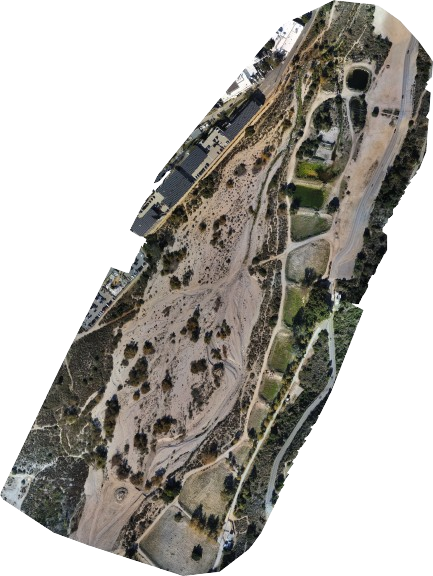
\includegraphics[scale=0.5]{images/evaluation/arroyo.png}
        \caption{Map of the Arroyo Seco area outside the Jet Propulsion Laboratory}
    \end{figure}
    \begin{figure}[h]
        \centering
        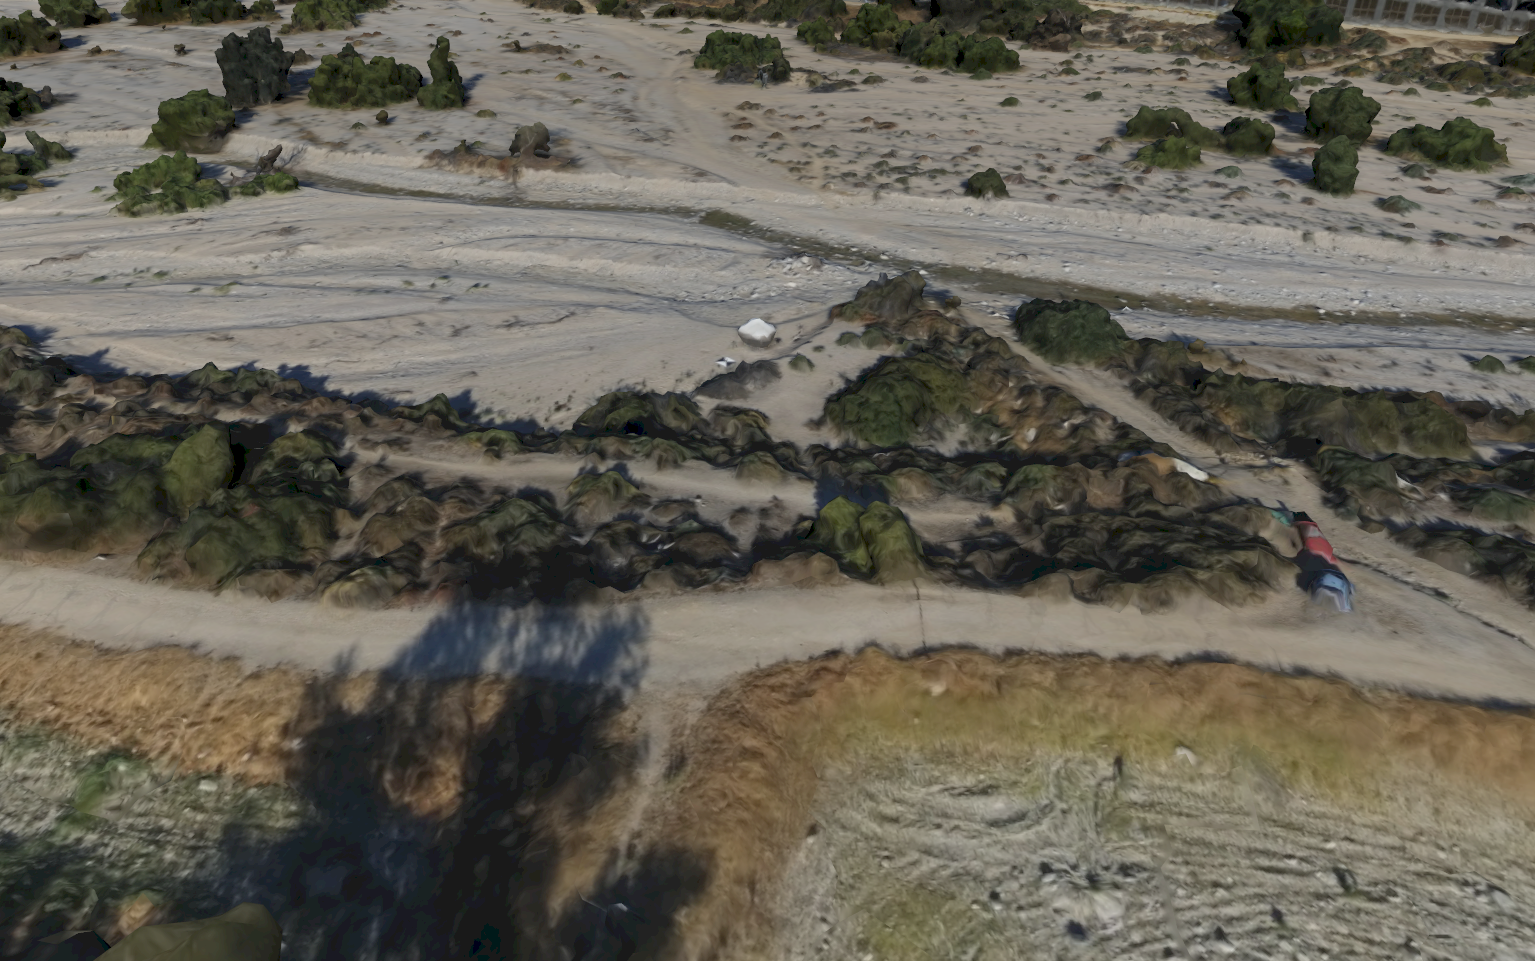
\includegraphics[scale=0.23]{images/evaluation/arroyo_map.png}
        \caption{Close Up of the Arroyo Map}
        \label{fig:sim_view_arroyo}
    \end{figure}
    \item Rough Test Map - A control environment designed to prevent LSD from detecting any landing site unless a landing platform is specifically spawned. It was created using blender and applying white noise perturbations to the elevation of a plane. Note that there is no texture projected onto the terrain. Therefore, on this map only ground truth was used.
    \begin{figure}[h]
        \centering
        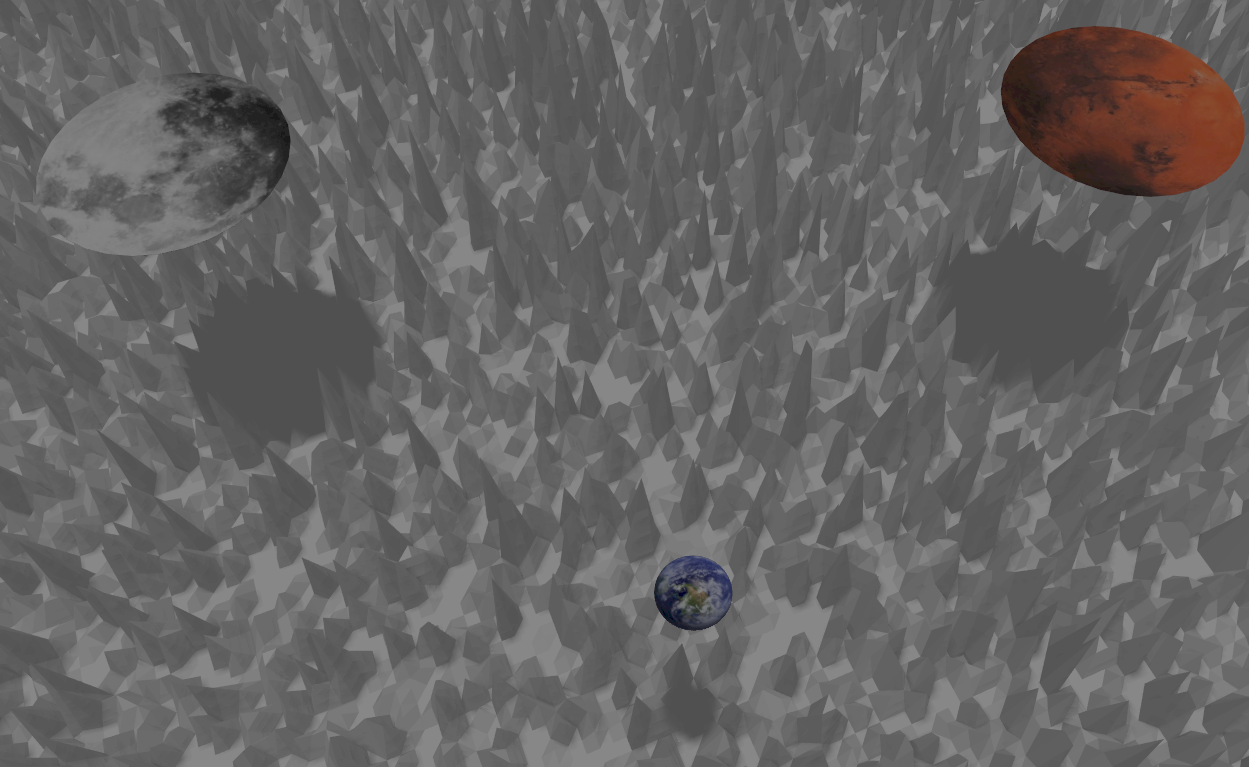
\includegraphics[scale=0.285]{images/evaluation/rough_test_map.png}
        \caption{Synthetically created map with no landing sites apart from inserted landing platforms.}
    \end{figure}
    \begin{figure}[h]
        \centering
        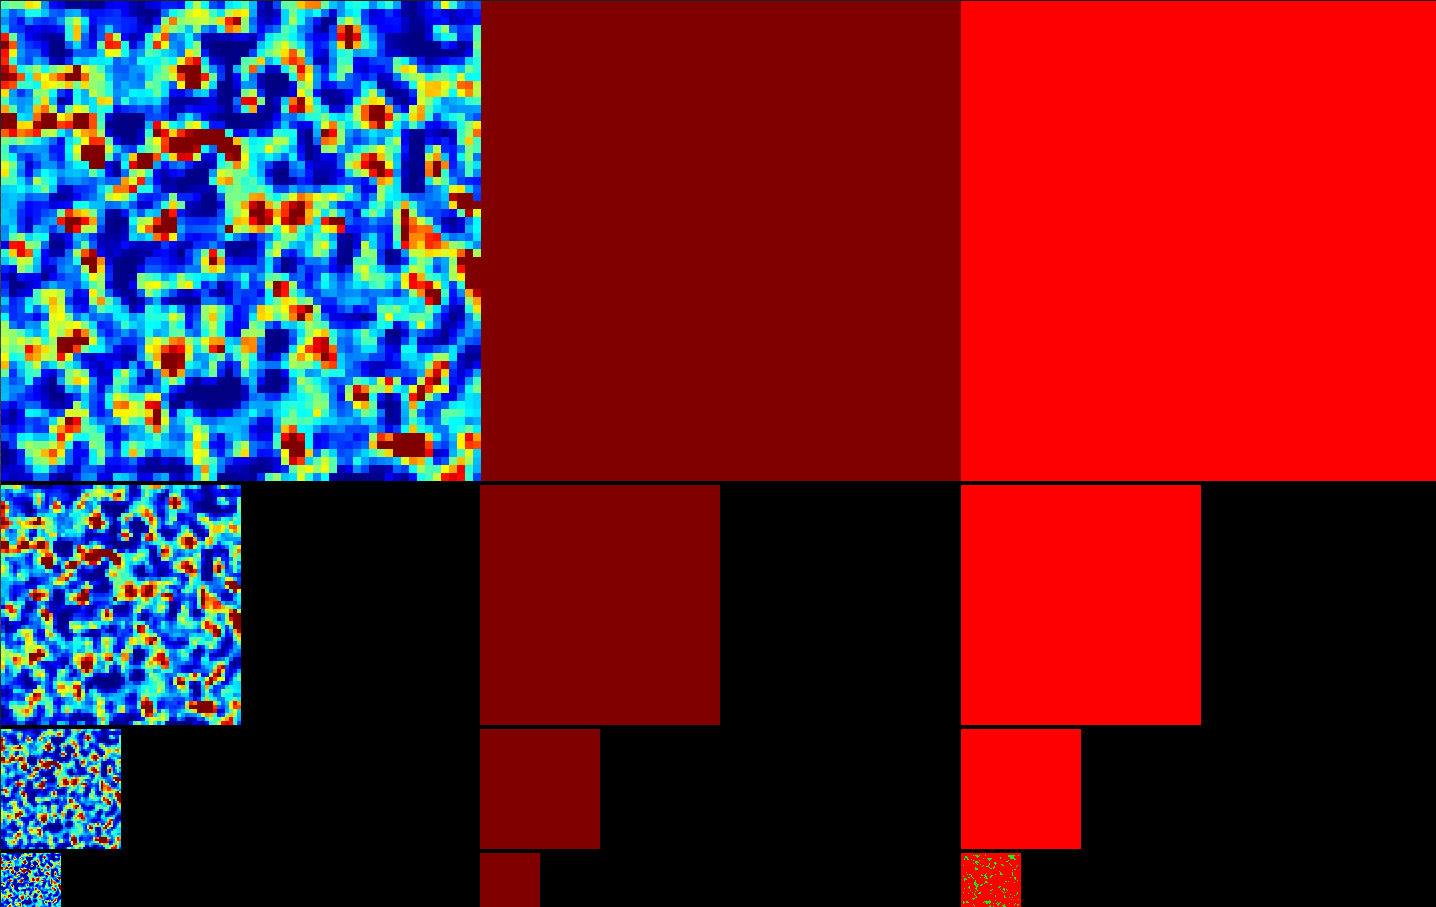
\includegraphics[scale=0.25]{images/evaluation/rough_map_LSD.png}
        \caption{LSD debug output shown of the plain rough environment}
    \end{figure}
    \begin{figure}[h]
        \centering
        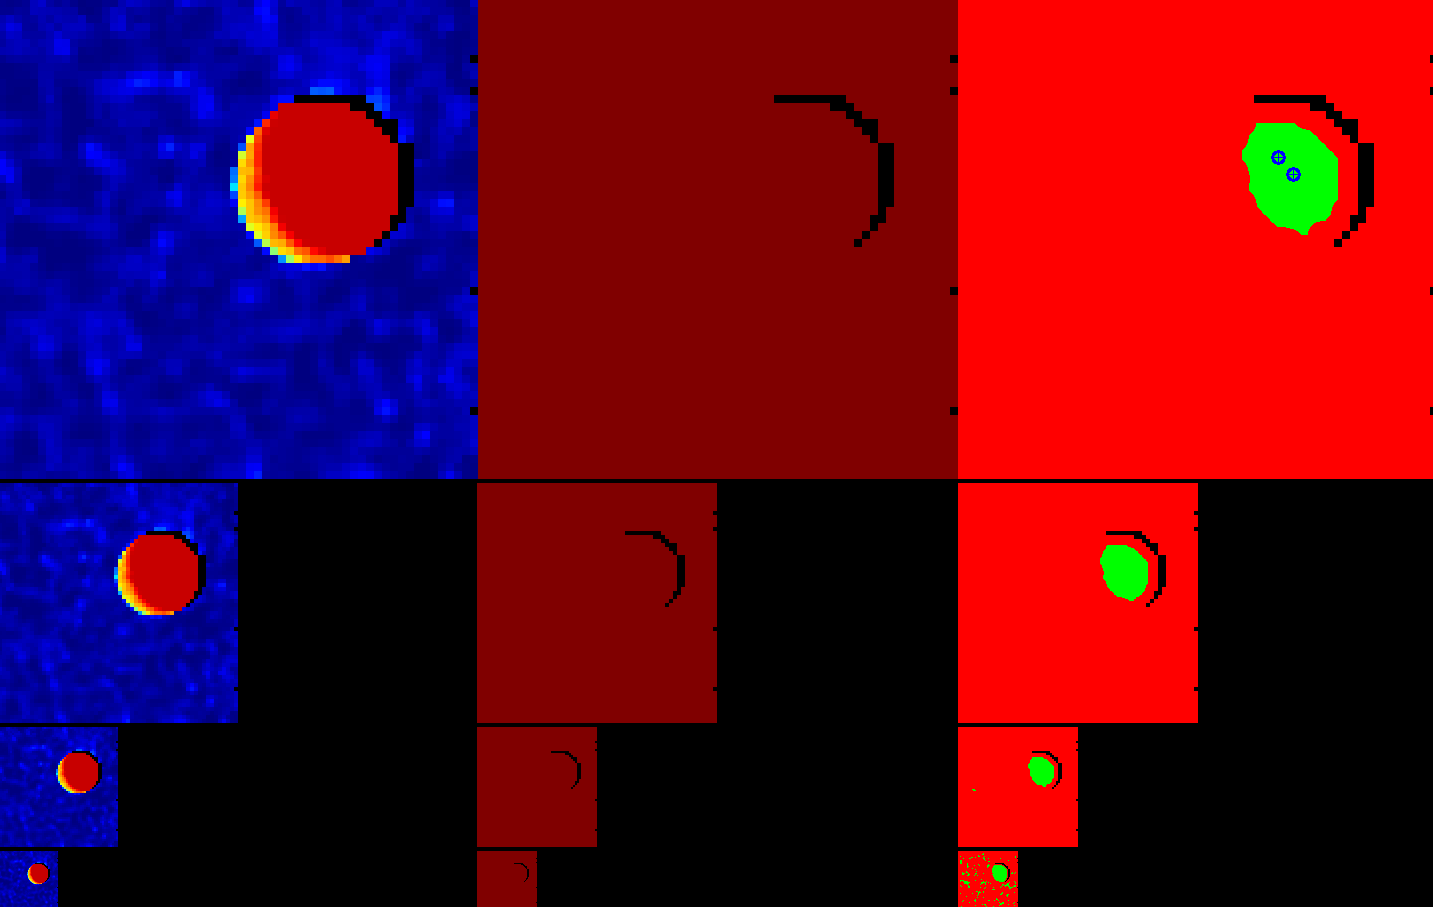
\includegraphics[scale=0.25]{images/evaluation/rough_map_LSD_platform.png}
        \caption{LSD debug image of the rough control map with spawned landing platforms}
    \end{figure}
\end{itemize}
\clearpage %HERE
\subsection{Drone Spawn}
The drone was either spawned repeatedly from a default location on the ground (The start location from when the actual fields tests were performed) or from a random location. For a simplicity way of  avoiding terrain collisions, the drone was spawned on a randomly positioned disk at 40 m altitude. The start disk's size was only 0.5 m in diameter which prevented it from being considered too good of a landing site by LSD. This is important because the platform implicitly gains quality due to the fact, that it is located higher up than the terrain, leading to a lower distance to the drone when flying at mission altitude.
\begin{figure}[h]
    \centering
    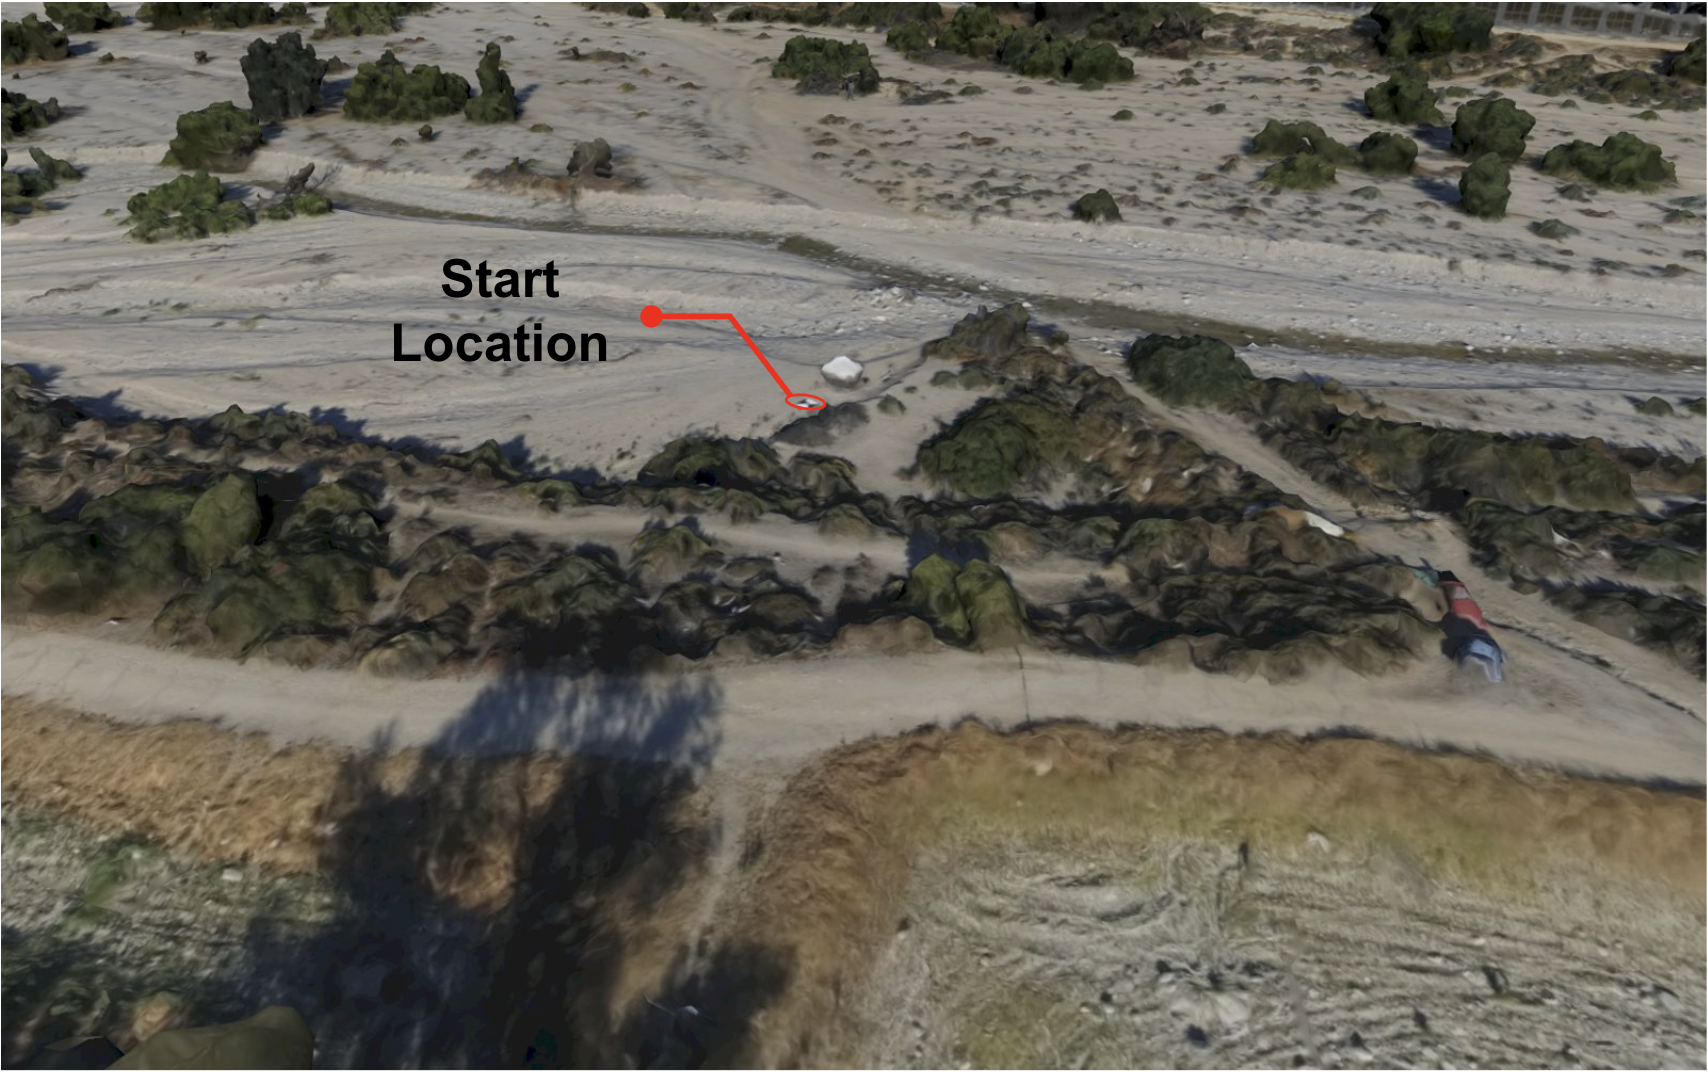
\includegraphics[scale=0.42]{images/evaluation/arroyo_with_start.png}
    \caption{Arroyo Map with Fixed Start Position}
    \label{fig:fixed_start}
\end{figure}
\begin{figure}[h]
    \centering
    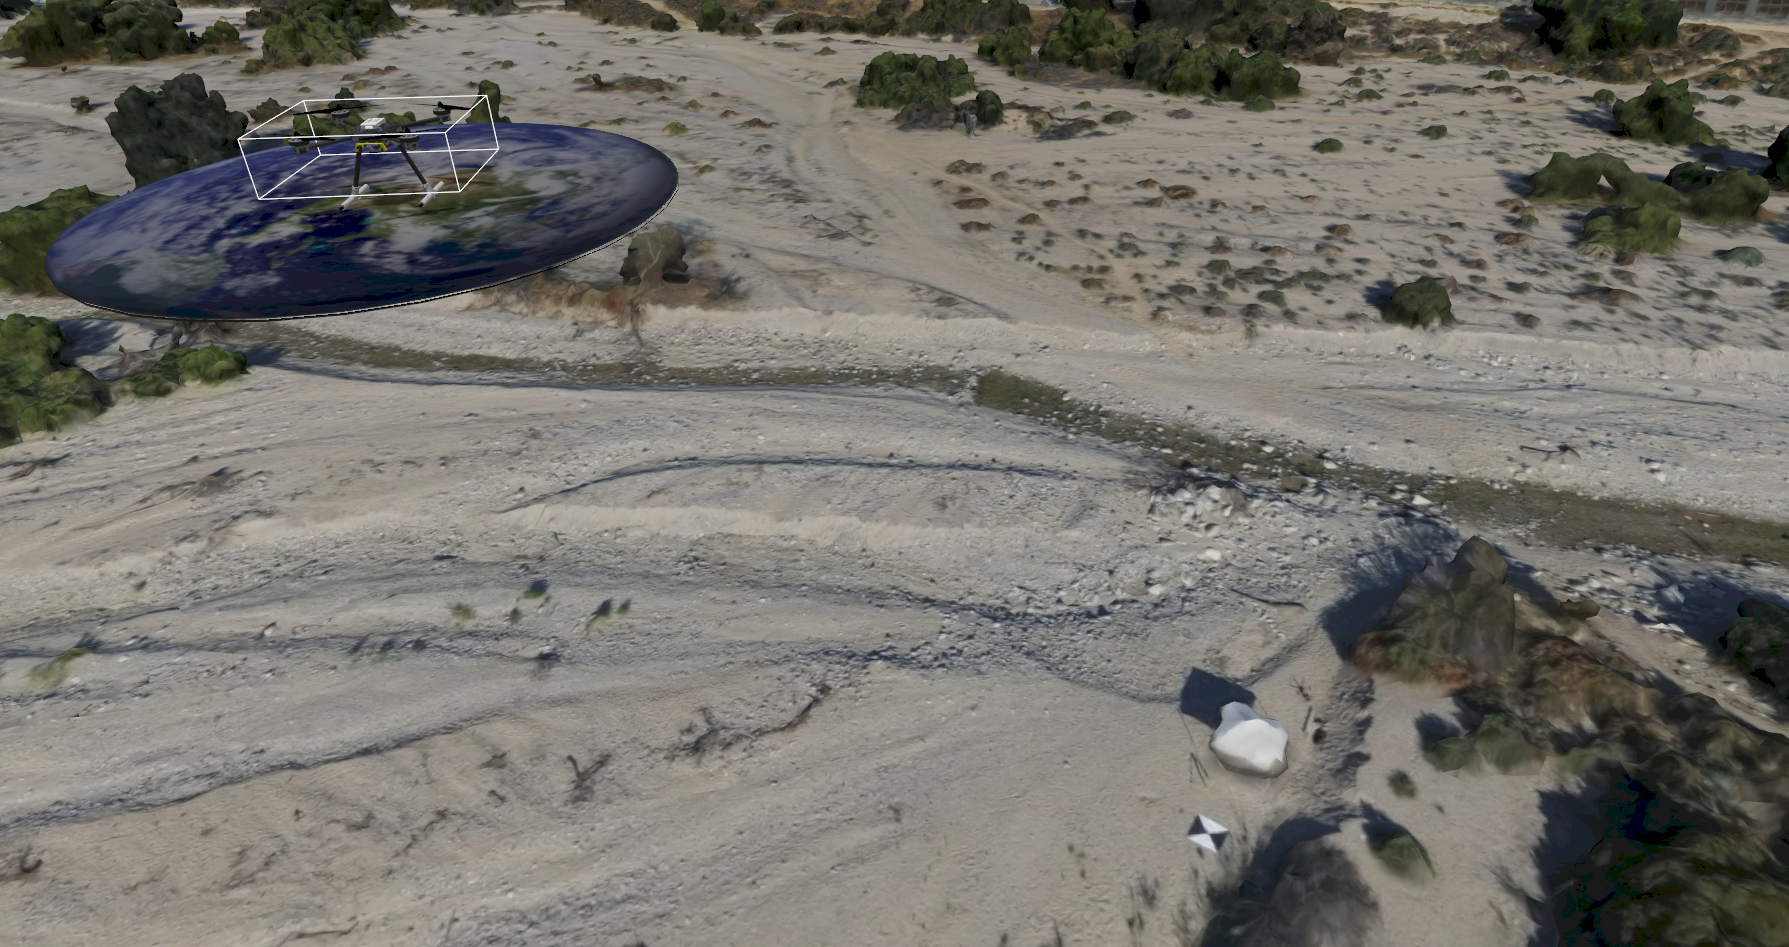
\includegraphics[scale=0.2]{images/evaluation/arroyo_with_platform.png}
    \caption{Arroyo map with randomly positioned spawn platform}
    \label{fig:random_start}
\end{figure}
\clearpage %HERE

\subsection{Depth Source}
As mentioned in \cref{sec:sfm_lsd_eval}, at the time of this work SFM was very fragile as an individual module. Because of this and to evaluate the merged pipeline as opposed to the depth generation module, ground truth depth was used at high altitudes unless specified otherwise. Regardless of whether ground truth or SFM was used, the verification at low altitudes was always performed using the point clouds from the stereo camera depth node.

\subsection{Success Conditions}
To determine whether a flight was successful or not, two main metrics were considered. First, whether the landing action in the autonomy was initiated (this happens only after the landing site selection and verification were both successful) and secondly to infer the safety of the rotorcraft, a rosbag was collected and analyzed to check whether either the roll or pitch value exceeded the crash threshold. In practice, a threshold of 1.2 radians or shortly below 70\degree proved to be an accurate decision boundary to detect a drone crash.

\subsubsection{Home Landings}
The drone lands at the home position in the two following cases:
\begin{itemize}
    \item No landing sites exist to be chosen.

    This happens when very few landing sites were detected yet failed verification and were therefore banned or when no landing sites were detected in the first place. 

    The latter case occurs in two scenarios: 
    \begin{itemize}
        \item The overflown terrain simply does not have a single landing site of decent quality. (see the rough map introduced in \cref{sec:exp_setup})
        \item The landing site detection algorithm failed to detect landing sites.
    \end{itemize}
    In both scenarios, going home is the desired behavior. However, if LSD does not detect landing sites, the run cannot be counted as a success regardless of whether the drone landed safely after taking off.

    Looking at the Arroyo map shown in \cref{fig:sim_view_arroyo} and speaking from development experience, sufficient landing sites should be found on this map. Therefore, landing at home when flying on the Arroyo indicates a landing site pipeline issue.
    \item A landing site is chosen at the home position.

    This is possible as the stereo camera detects landing sites on the takeoff location when ascending. However, given that the last mission waypoint is sufficiently far away from the takeoff location, the drone should land at a closer location. 
\end{itemize}


\subsection{Visual Analysis}
To further analyze the randomized flights in a bit more detail, visual landing attempt projections are used. Such an analysis image is shown in \cref{fig:landing_attempts_dummy}.

\begin{figure}[h]
    \begin{center}
        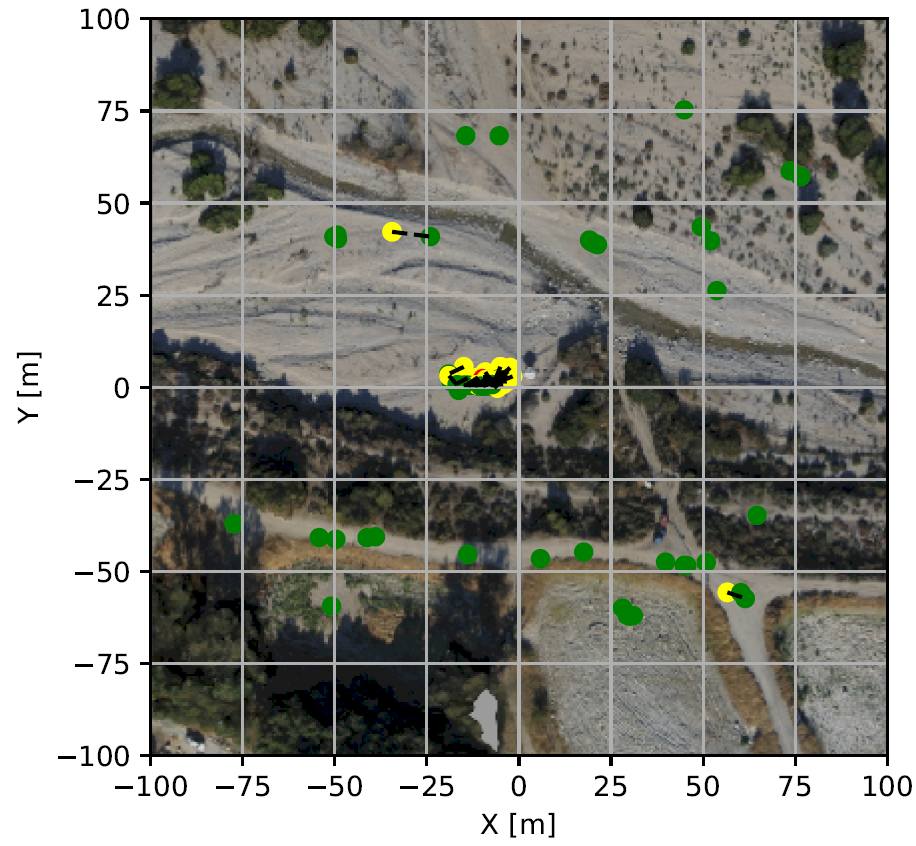
\includegraphics[scale=0.5]{images/evaluation/landings_random_WP_GT.png}
        \caption{Landing Attempt dummy image - Green: successful landing, Yellow: verification failure, Blue: landing at home position}
        \label{fig:landing_attempts_dummy}
    \end{center}
\end{figure}

The green points indicate successful verifications which lead to the initiation of the landing action shortly after. (If no rotation above a failure threshold was detected, this is considered a successful landing.) 

The yellow points are landing attempts, where a chosen landing site was not verified and thus banned from further consideration. It is crucial to note that not being able to verify a landing site is no issue at all. Landing sites detected at high altitudes merely provide a preliminary indication of potential landing zones. It is the subsequent phase, responsible for verifying these sites, that yields the refined final landing site knowledge used for landing. So selecting a landing site at high altitude, not being able to verify it and subsequently choosing a close by landing site detected during verification might even be called the most promising chain of actions in the pursuit of autonomous landing.

Lastly, blue points indicate successful landings achieved through the trigger of the landing-at-home action. As previously mentioned, When flying on a map with obvious landing opportunities, triggering the landing-at-home action indicates an issue with the landing site detection mechanism.

In the case of multiple attempts at verifying a landing site, connection lines are drawn between the failed attempts and the final landing indicating which subsequent sites were chosen.

% TODO: maybe add the circles of spawn and home and describe them

\subsection{Off Board Mode connection Issues}
As will be presented in the following, connection failures between the PX4 flight controller and the autonomy occurred, leading to the deactivation of the off board mode and therefore the loss of control of the autonomy over the rotorcraft. These issues arose most likely because the MAVROS connection in between failed to send a necessary heartbeat repeatedly and thus the connection was intercepted.

Self-evidently, this did not result in a successful landing and was not counted as such. However, as these connection issues did not occur due to insufficiencies in the pipeline presented in this work, they were not considered failures of the pipeline either.
\clearpage
\section{Test Flights}\label{sec:test_flights}
\subsection{Arroyo - Randomized Waypoints}\label{subsec:eval_rand_wp}

When starting 100 times from the fixed position indicated in \cref{fig:fixed_start} and flying to random mission waypoints at 100 m altitude in a 70x70m vicinity on the Arroyo map, the following results were achieved:

\begin{table}[h]
    \begin{center}
     \caption{Results with fixed takeoff and random waypoint}\vspace{1ex}
     \label{tab:result_random_waypoint}
     \begin{tabular}{|c|c|c|c|c|}
     \hline
     \# Flights & \# Successes & \# Timeouts & \# Crashes & \# Home Landing\\ \hline \hline
     100 & 99 & 1 & 0 & 0 \\
     \hline
     \end{tabular}
    \end{center}
    \end{table}

    The landing attempt numerics are shown here:
    \begin{table}[h]
        \begin{center}
         \caption{Landing attempts with fixed takeoff and random waypoint}\vspace{1ex}
         \label{tab:land_nums_random_waypoint}
         \begin{tabular}{|c|c|c|c|}
         \hline
         \# Flights & \# Landing on first attempt & \# 2 attempts & \# 3 attempts\\ \hline \hline
         100 & 48 & 45 & 7 \\
         \hline
         \end{tabular}
        \end{center}
    \end{table}

    \begin{figure}[h]
        \begin{center}
            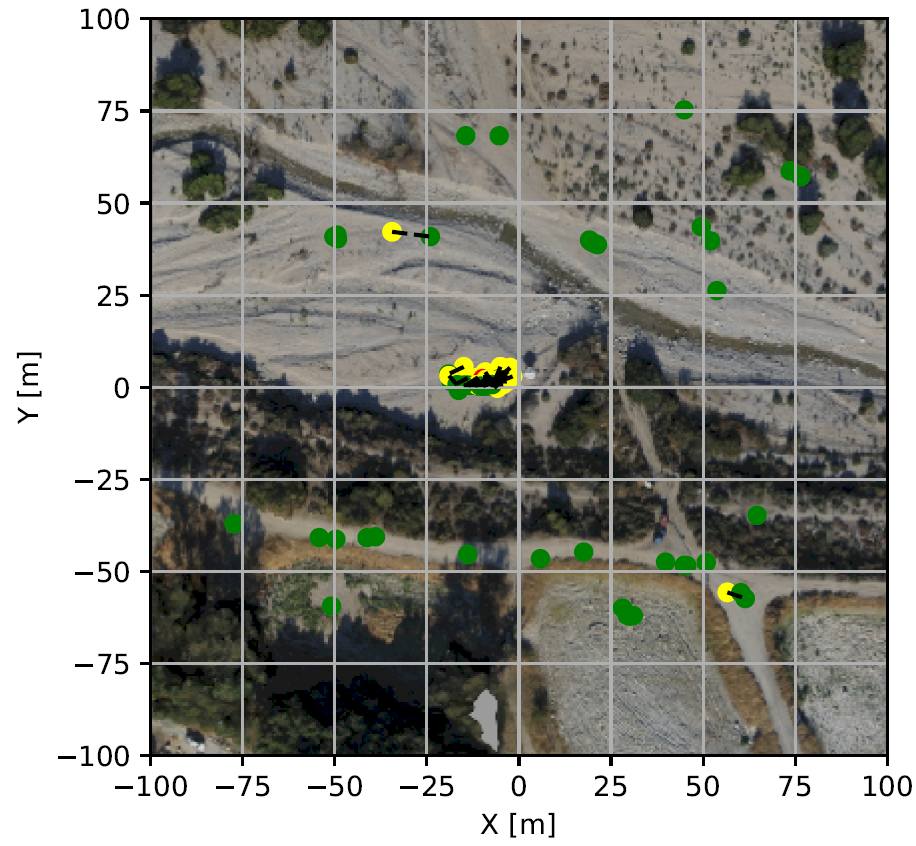
\includegraphics[scale=0.5]{images/evaluation/landings_random_WP_GT.png}
            \caption{Landing Attempts - Green: successful landing, Yellow: verification failure, Blue: landing at home position}
            \label{fig:landing_attempts_random_WP}
        \end{center}
    \end{figure}

    \subsubsection{Numeric Discussion}
    \cref{tab:result_random_waypoint} shows the numeric outcome of the flights. 1 timeout occurred but each performed flight by the autonomy was a success, landing safely and controlled. No home landings were necessary which, as described above, indicates a very robust LSD performance. A high number of flights where two landing site verification attempts were performed is also well within acceptable boundaries because the first landing site might as well be used as an indicator to draw the drone closer to an area where high quality sites can be detected using the stereo camera.

    \subsubsection{Visual Discussion}
    Let's consider the landing image \ref{fig:landing_attempts_random_WP}. The final landing sites indicated in green span exclusively decent landing areas. The verification attempts that fell short are indicated with yellow and annotated by a line connection to the successful attempt thereafter. Subsequent landing sites were always detected short distances away from failed candidates which is exactly the correct behavior in order to not lose time pursuing a far away landing site. As indicated in \cref{subsec:heuristics} this is thanks to the verification altitude which incentivizes the selection of other landing sites detected at the current verification altitude. Lastly the attempt which timed out is hardly visible indicated in red. %TODO: make appendix with autonomy log of failed runs and show timeout.

    The last thing to mention is the clustering of the landing sites around the takeoff location. The reason for this is twofold:
    \begin{itemize}
        \item \textbf{Quality}: The takeoff position was also the takeoff position for the physical flights in performed in the field. It was chosen exactly because of its even and smooth characteristics. Therefore, it is no surprise that many landing sites were detected around that location.
        \item \textbf{OMG Conversion}: During ascent, when using either stereo or ground truth depth, the same area is perceived repeatedly. This leads to a convergence in certainty in the map aggregation step of LSD. As landing sites have a higher chance of being detected on terrain with a low uncertainty, the takeoff position is most likely selected until it leaves the rolling buffer map.
    \end{itemize}

    This test is a very clear demonstration of the applied chosen heuristics. The best landing site detected is very likely one that is detected at the takeoff position. Around this clustering of landings there is notable space of no attempts performed. This can be attributed to the competing motives of the landing site selection. The quality of the landing site defines the autonomy's choice until the drone's distance to that landing site is too big, and a closer one is chosen. 

\subsection{Arroyo - Randomized Takeoff and Waypoints}\label{subsec:compl_rand}

    In this set of test flights, randomized takeoff positions were used as shown in \cref{fig:random_start}. Missions were built using a randomized waypoint in a 70x70m surrounding.

    The numerical results look as follows:

    \begin{table}[h]
        \begin{center}
         \caption{Results with random takeoff location and random waypoint}\vspace{1ex}
         \label{tab:result_complete_rand}
         \begin{tabular}{|c|c|c|c|c|}
         \hline
         \# Flights & \# Successes & \# Timeouts & \# Crashes & \# Home Landing\\ \hline \hline
         100 & 99 & 1 & 0 & 0 \\
         \hline
         \end{tabular}
        \end{center}
    \end{table}
    \begin{table}[h]
        \begin{center}
         \caption{Landing attempts with random takeoff and random waypoint}\vspace{1ex}
         \label{tab:land_nums_complete_rand}
         \begin{tabular}{|c|c|c|c|c|}
         \hline
         \# Flights & \# 1 attempt & \# 2 attempts & \# 3 attempts & \# 4 attempts\\ \hline \hline
         100 & 78 & 15 & 5 & 2 \\
         \hline
         \end{tabular}
        \end{center}
    \end{table}

    And the visual outcome:

    \begin{figure}[h]
        \begin{center}
            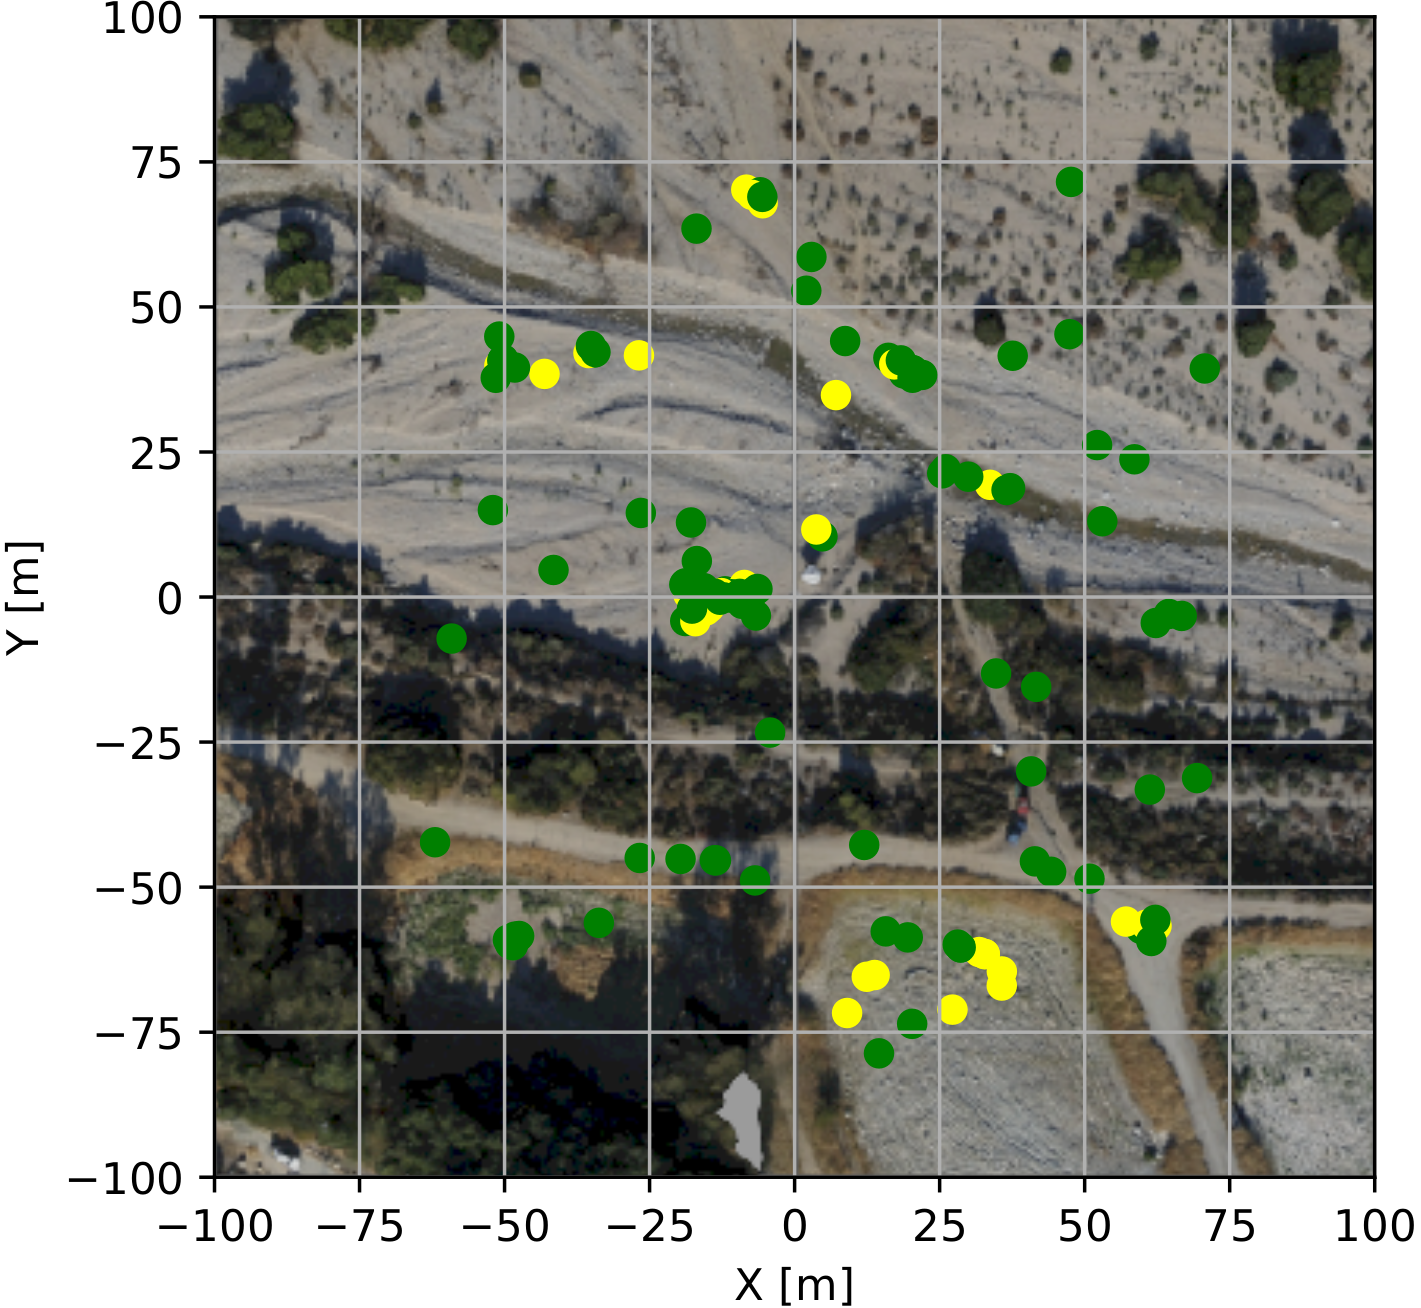
\includegraphics[scale=0.25]{images/evaluation/landings_complete_randomized_GT.png}
            \caption{Landing attempts with randomized drone spawn - Green: successful landing, Yellow: verification failure, Blue: landing at home position}
            \label{fig:landing_attempts_complete_rand}
        \end{center}
    \end{figure}

    \subsubsection{Numeric Discussion}
    Exactly the same success rate was reached as in \cref{subsec:eval_rand_wp}. Notably however, many more attempts landed at the first site considered. %TODO why is that?


    \subsubsection{Visual Discussion}
    Compared to \cref{fig:landing_attempts_random_WP}, the landing attempts are more spread out over the map. Fewer landings were attempted at the takeoff position. This is the case because the area wasn't always covered by the mission's trajectory and the flights spent less time above that area as the drone spawned randomly. Thus, the pipeline did not converge at that location leading to a smaller chance of landing sites being detected there. As for the fixed spawn location, the second attempts were always at landing sites close by which is desirable.

\subsection{Rough Map - Random Waypoints over Platforms}\label{subsec:rough_coverage}
        \begin{figure}[h]
            \centering
            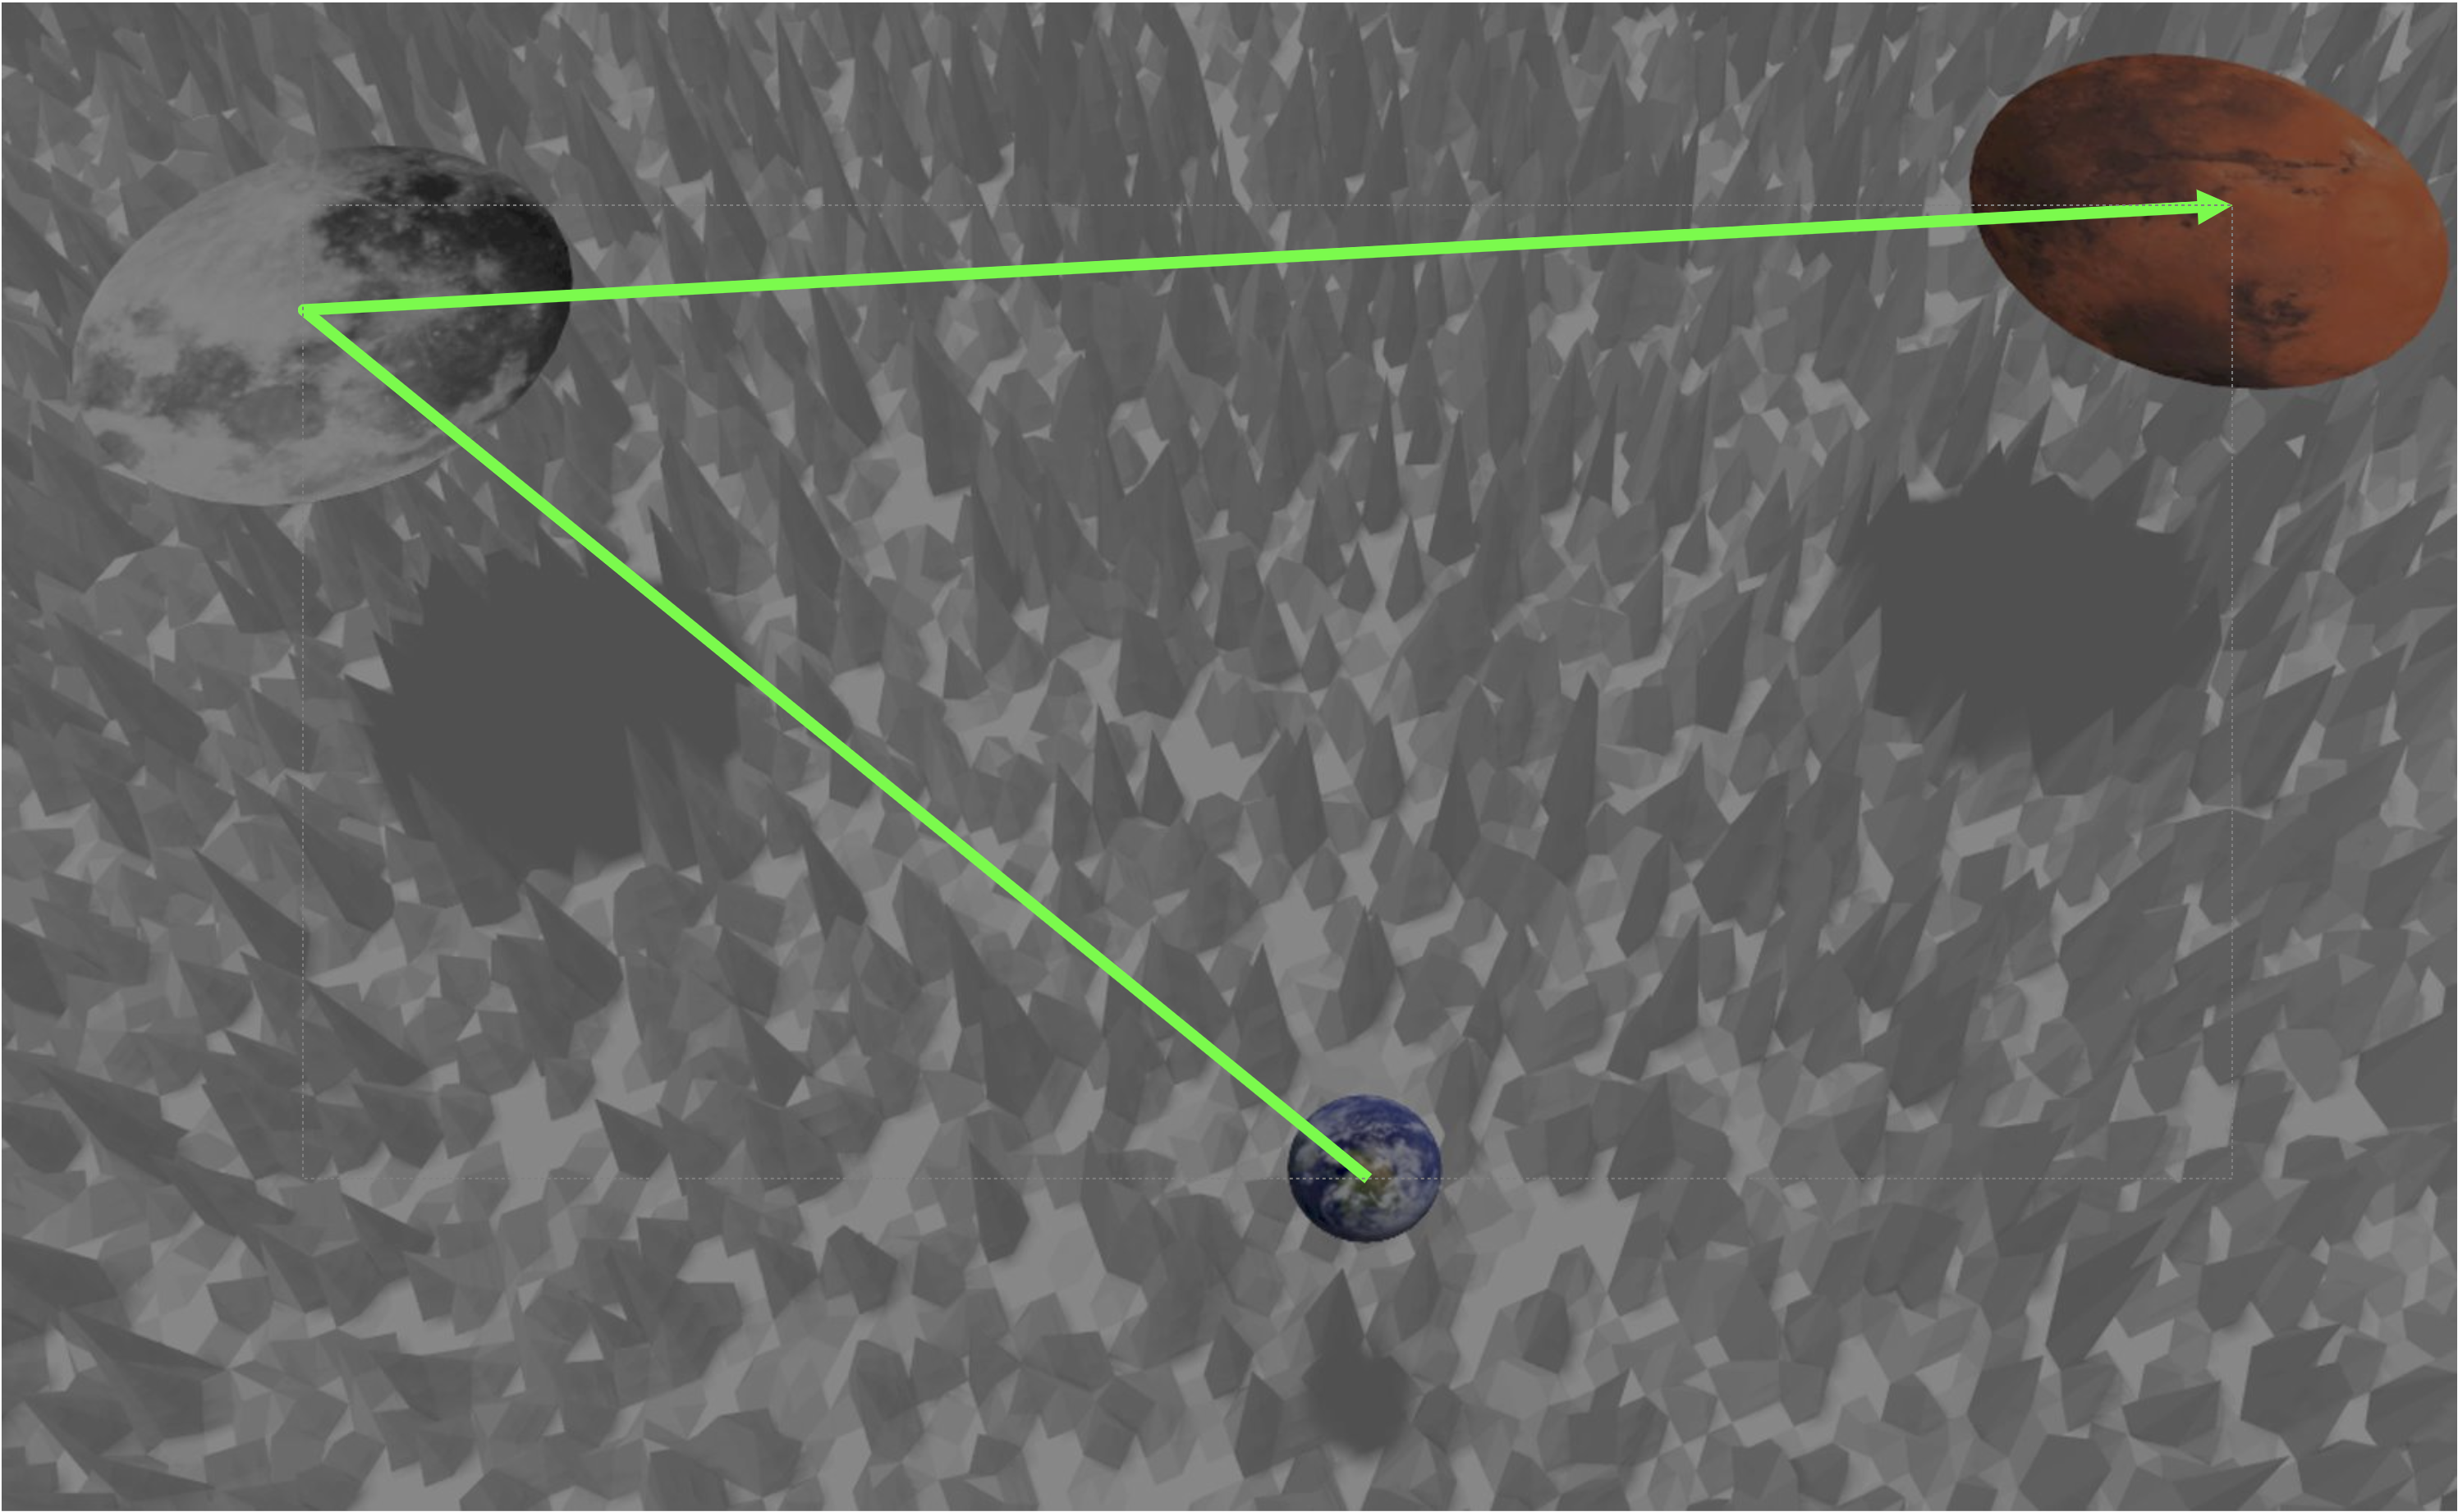
\includegraphics[scale=0.24]{images/evaluation/rough_over_platforms.png}
            \caption{Test flights on rough map with waypoints covering the landing sites}
            \label{fig:rough_covered}
        \end{figure}

        In this test, the drone flew a randomized two-waypoint pattern which always covered the synthetically added landing platforms. The idea behind this experiment was to eliminate other landing possibilities and test, whether the approach at hand would be able to detect the controlled good landing sites.

        The numerical result thereof is displayed below:

        \begin{table}[h]
            \begin{center}
             \caption{Results - Rough map with platform coverage}\vspace{1ex}
             \label{tab:result_rough_covered}
             \begin{tabular}{|c|c|c|c|c|}
             \hline
             \# Flights & \# Successes & \# Timeouts & \# Crashes & \# Home Landing\\ \hline \hline
             20 & 19 & 1 & 0 & 0 \\
             \hline
             \end{tabular}
            \end{center}
        \end{table}

        \begin{table}[h]
            \begin{center}
             \caption{Landing attempts rough map with platform covering mission}\vspace{1ex}
             \label{tab:land_nums_rough_coverage}
             \begin{tabular}{|c|c|c|c|}
             \hline
             \# Flights & \# Landing on first attempt & \# 2 attempts & \# 3 attempts\\ \hline \hline
             20 & 20 & 0 & 0 \\
             \hline
             \end{tabular}
            \end{center}
        \end{table}

        \begin{figure}[h]
        \centering
        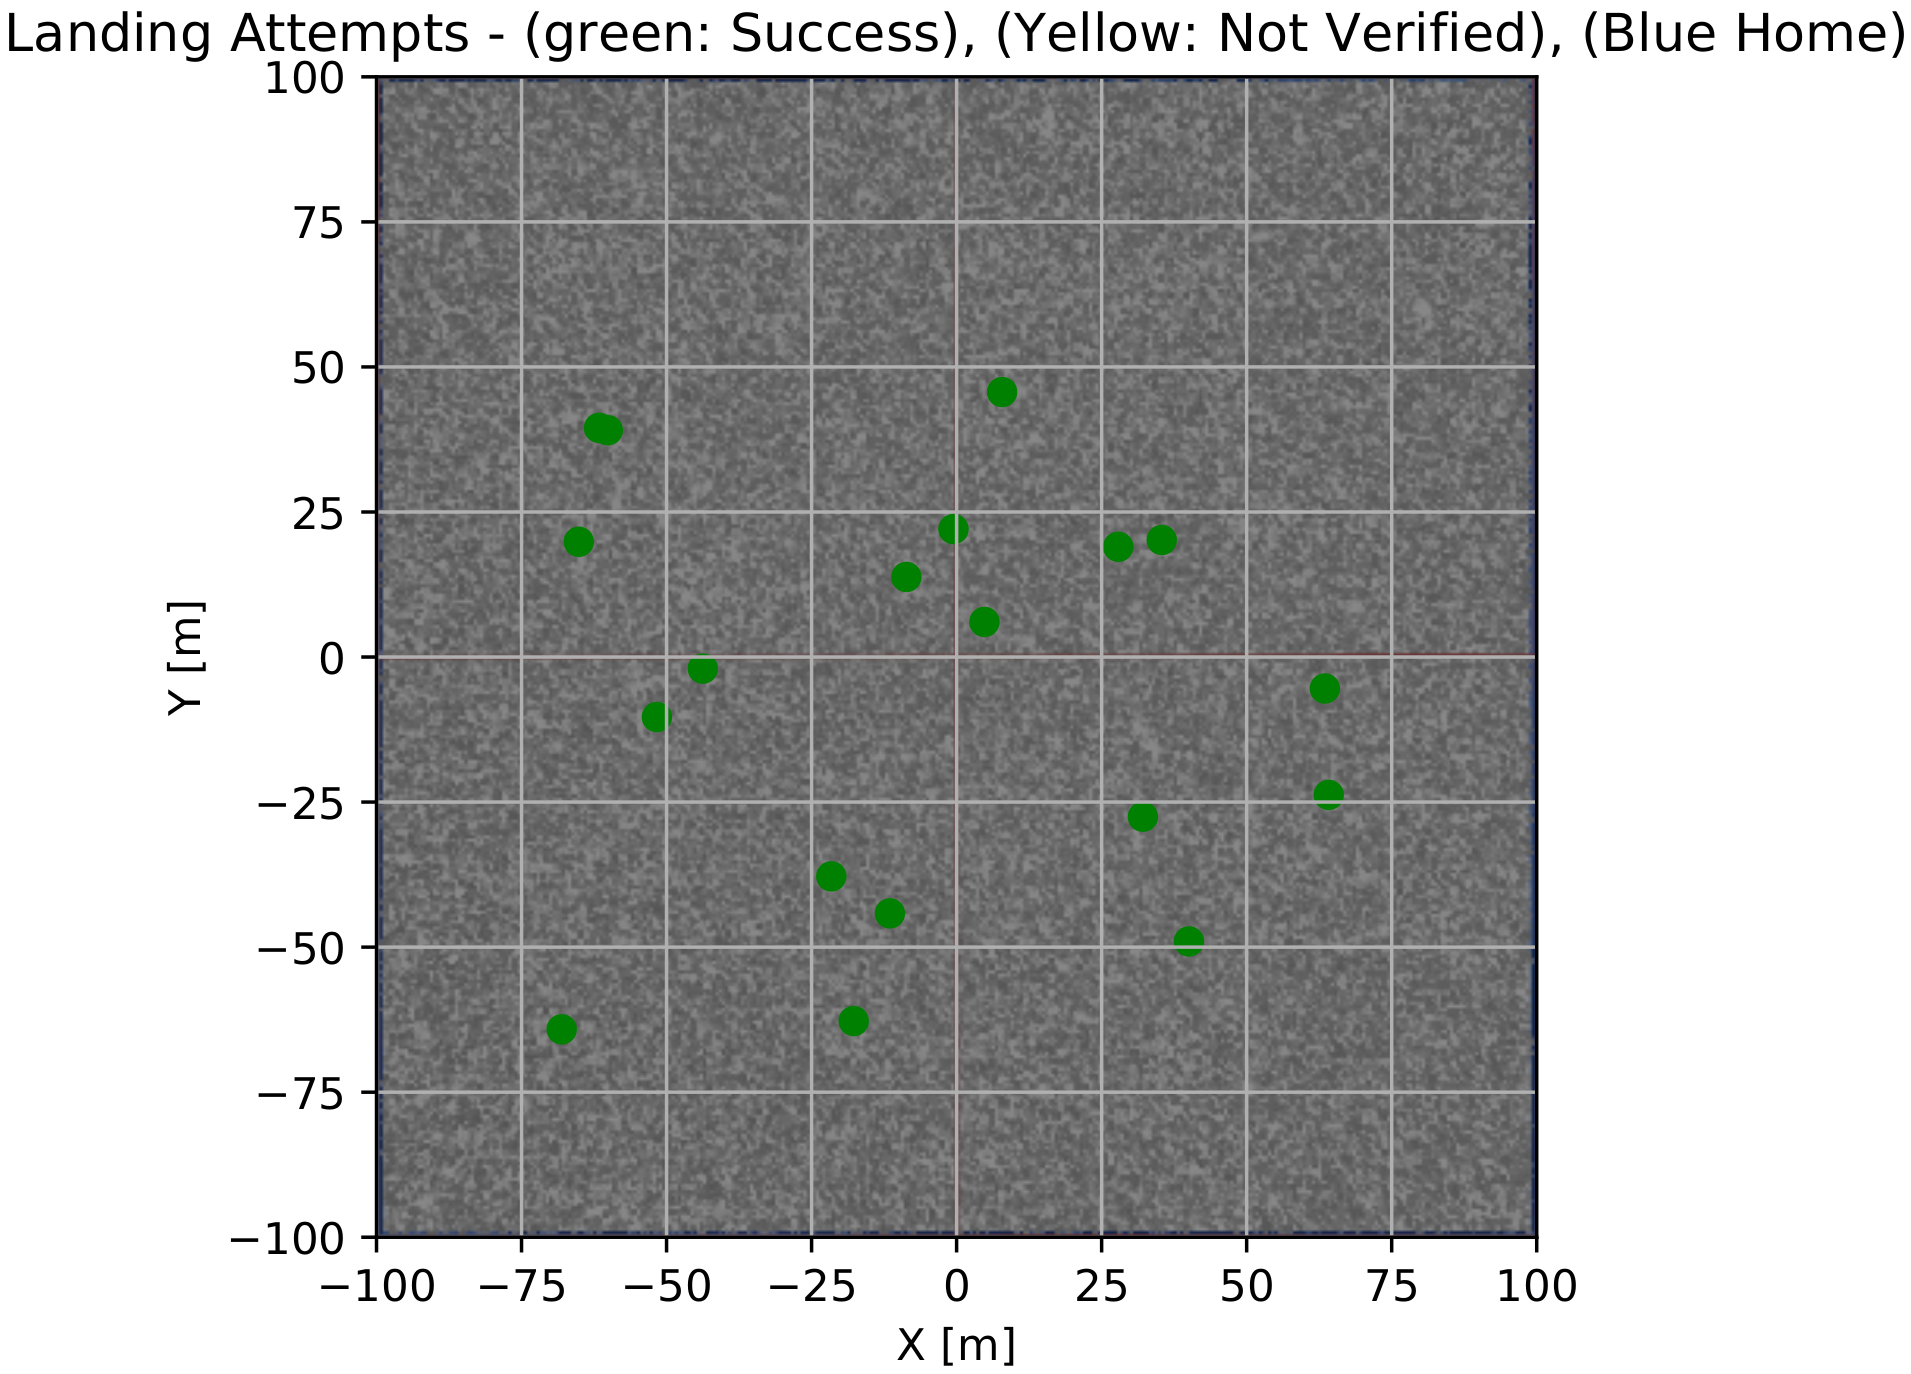
\includegraphics[scale=0.5]{images/evaluation/landing_rough_covered.png}
        \caption{Landing attempt locations for the rough map with platform covered by the mission}
        \label{fig:land_rough_covered}
        \end{figure}

        As both the spawn platform and the landing platforms where spawned randomly, evaluating the visual outcome is redundant. For sake of completion however, it is still displayed.

        \subsubsection{Numerical Discussion}
        One timeout occurred, but each attempt at landing resulted in a success. 

        This proves that LSD does in fact not perceive convincing landing sites where there should be none. Additionally, as the drone never went home, this proves that LSD also detects landing sites where there should be safe landing zones.
        
        Each landing site selected was verified. This convincing result is not surprising as the inserted landing sites are perfect landing sites and are therefore unlikely to trigger a verification failure.

\subsection{Rough Map - Completely Random Waypoints}

    \begin{figure}[h]
        \centering
        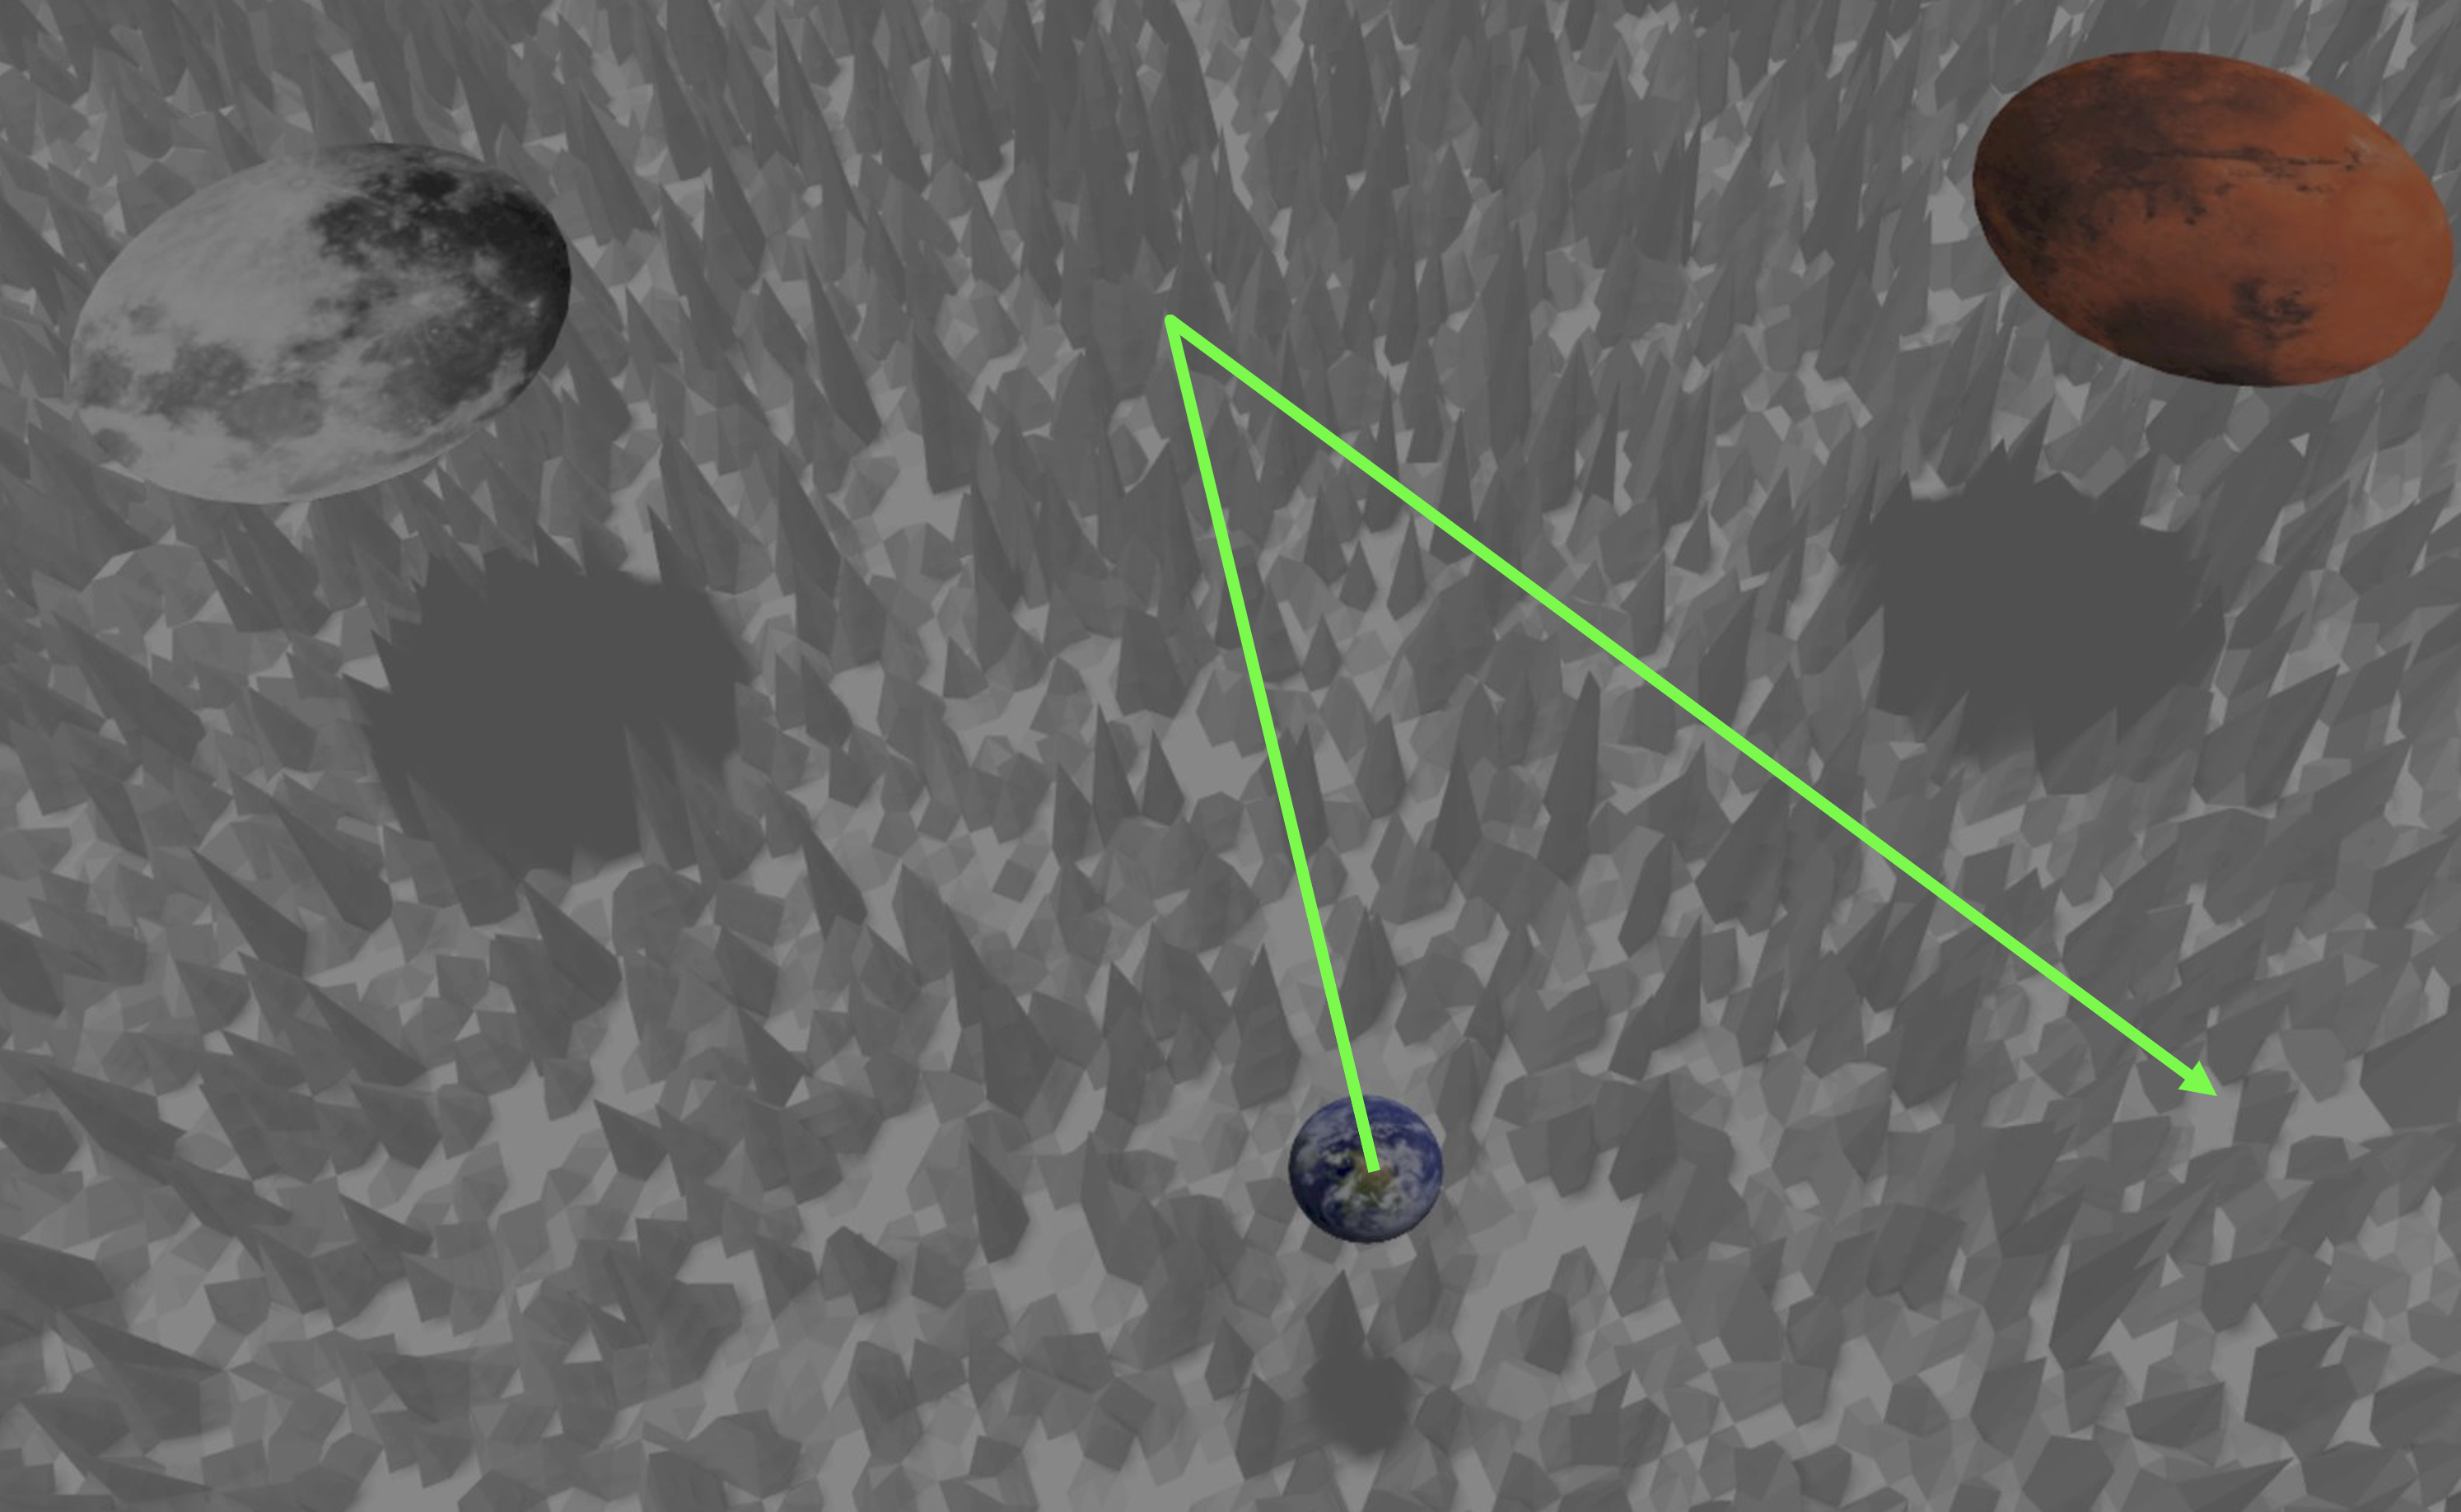
\includegraphics[scale=0.24]{images/evaluation/rough_complete_rand.png}
        \caption{Test flights on rough map with waypoints covering the landing sites}
        \label{fig:rough_compl_rand}
    \end{figure}

    Changing the setup a bit, in this test, the drone flew a completely randomized two-waypoint pattern without the guarantee of flying over a safe landing site. This test set analyzed the pipeline's capabilities to deal with the case when no landing sites are detected initially.

    The numerical result thereof is displayed below:

    \begin{table}[h]
        \begin{center}
         \caption{Results - Rough map with platform coverage}\vspace{1ex}
         \label{tab:result_rough_rand}
         \begin{tabular}{|c|c|c|c|c|}
         \hline
         \# Flights & \# Successes & \# Timeouts & \# Crashes & \# Home Landing\\ \hline \hline
         20 & 19 & 1 & 0 & 6 \\
         \hline
         \end{tabular}
        \end{center}
    \end{table}

    \begin{table}[h]
        \begin{center}
         \caption{Landing attempts rough map without platform covering mission}\vspace{1ex}
         \label{tab:land_nums_rough_rand}
         \begin{tabular}{|c|c|c|c|}
         \hline
         \# Flights & \# Landing on first attempt & \# 2 attempts & \# 3 attempts\\ \hline \hline
         20 & 13 & 1 & 0 \\
         \hline
         \end{tabular}
        \end{center}
    \end{table}

    \begin{figure}[h]
    \centering
    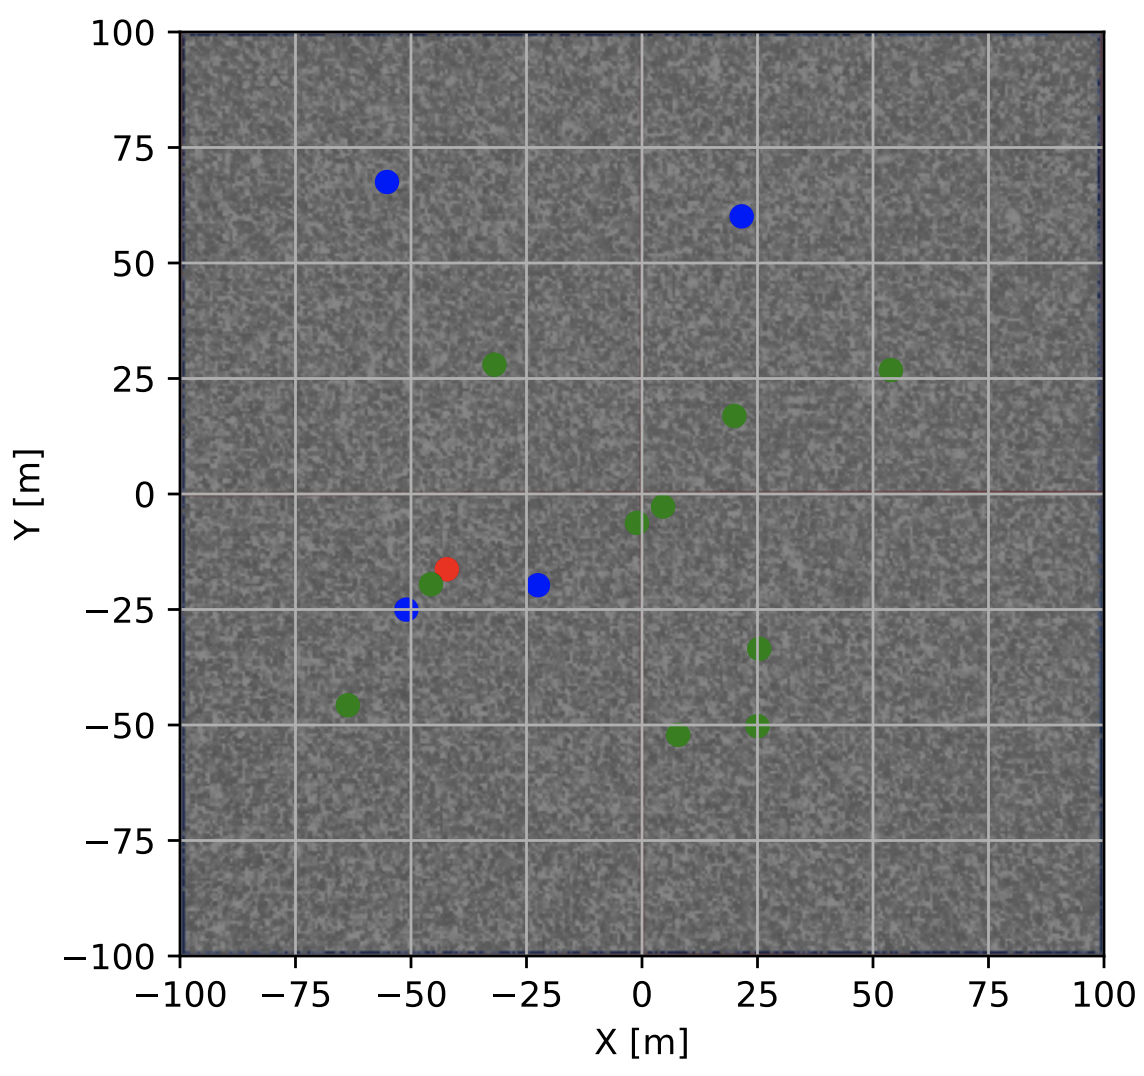
\includegraphics[scale=0.5]{images/evaluation/landing_rough_rand.png}
    \caption{Landing attempt locations for the rough map with completely random missions}
    \label{fig:land_rough_rand}
    \end{figure}

    \subsubsection{Numerical Discussion}

    Notably, the drone went to the home position 6 times. This is the desired behavior, when no landing site was found and is therefore to be considered a success. Like for the case when the platforms were covered by the mission, the landing sites were always verified as they were by design of high quality. One timeout remained also in this run.
    
    %TODO analyze also how many lses were found using the additional patterns.

% \subsection{Arroyo - Randomized Takeoff and Waypoints flown with SFM}\label{subsec:SFM_complete_rand}

    In this test the setup was the same as for \cref{subsec:compl_rand} with the exception, that SFM was used for the depth generation.

    The numerical result thereof is displayed below:

    \begin{table}[h]
        \begin{center}
            \caption{Results - Rough map with platform coverage}\vspace{1ex}
            \label{tab:result_rough_covered}
            \begin{tabular}{|c|c|c|c|c|}
            \hline
            \# Flights & \# Successes & \# Timeouts & \# Crashes & \# Home Landing\\ \hline \hline
            20 & 19 & 1 & 0 & 0 \\ %TODO: replace with values
            \hline
            \end{tabular}
        \end{center}
    \end{table}

    \begin{table}[h]
        \begin{center}
            \caption{Landing attempts rough map with platform covering mission}\vspace{1ex}
            \label{tab:land_nums_rough_coverage}
            \begin{tabular}{|c|c|c|c|}
            \hline
            \# Flights & \# Landing on first attempt & \# 2 attempts & \# 3 attempts\\ \hline \hline
            20 & 20 & 0 & 0 \\%TODO: replace
            \hline
            \end{tabular}
        \end{center}
    \end{table}

    \begin{figure}[h]
    \centering
    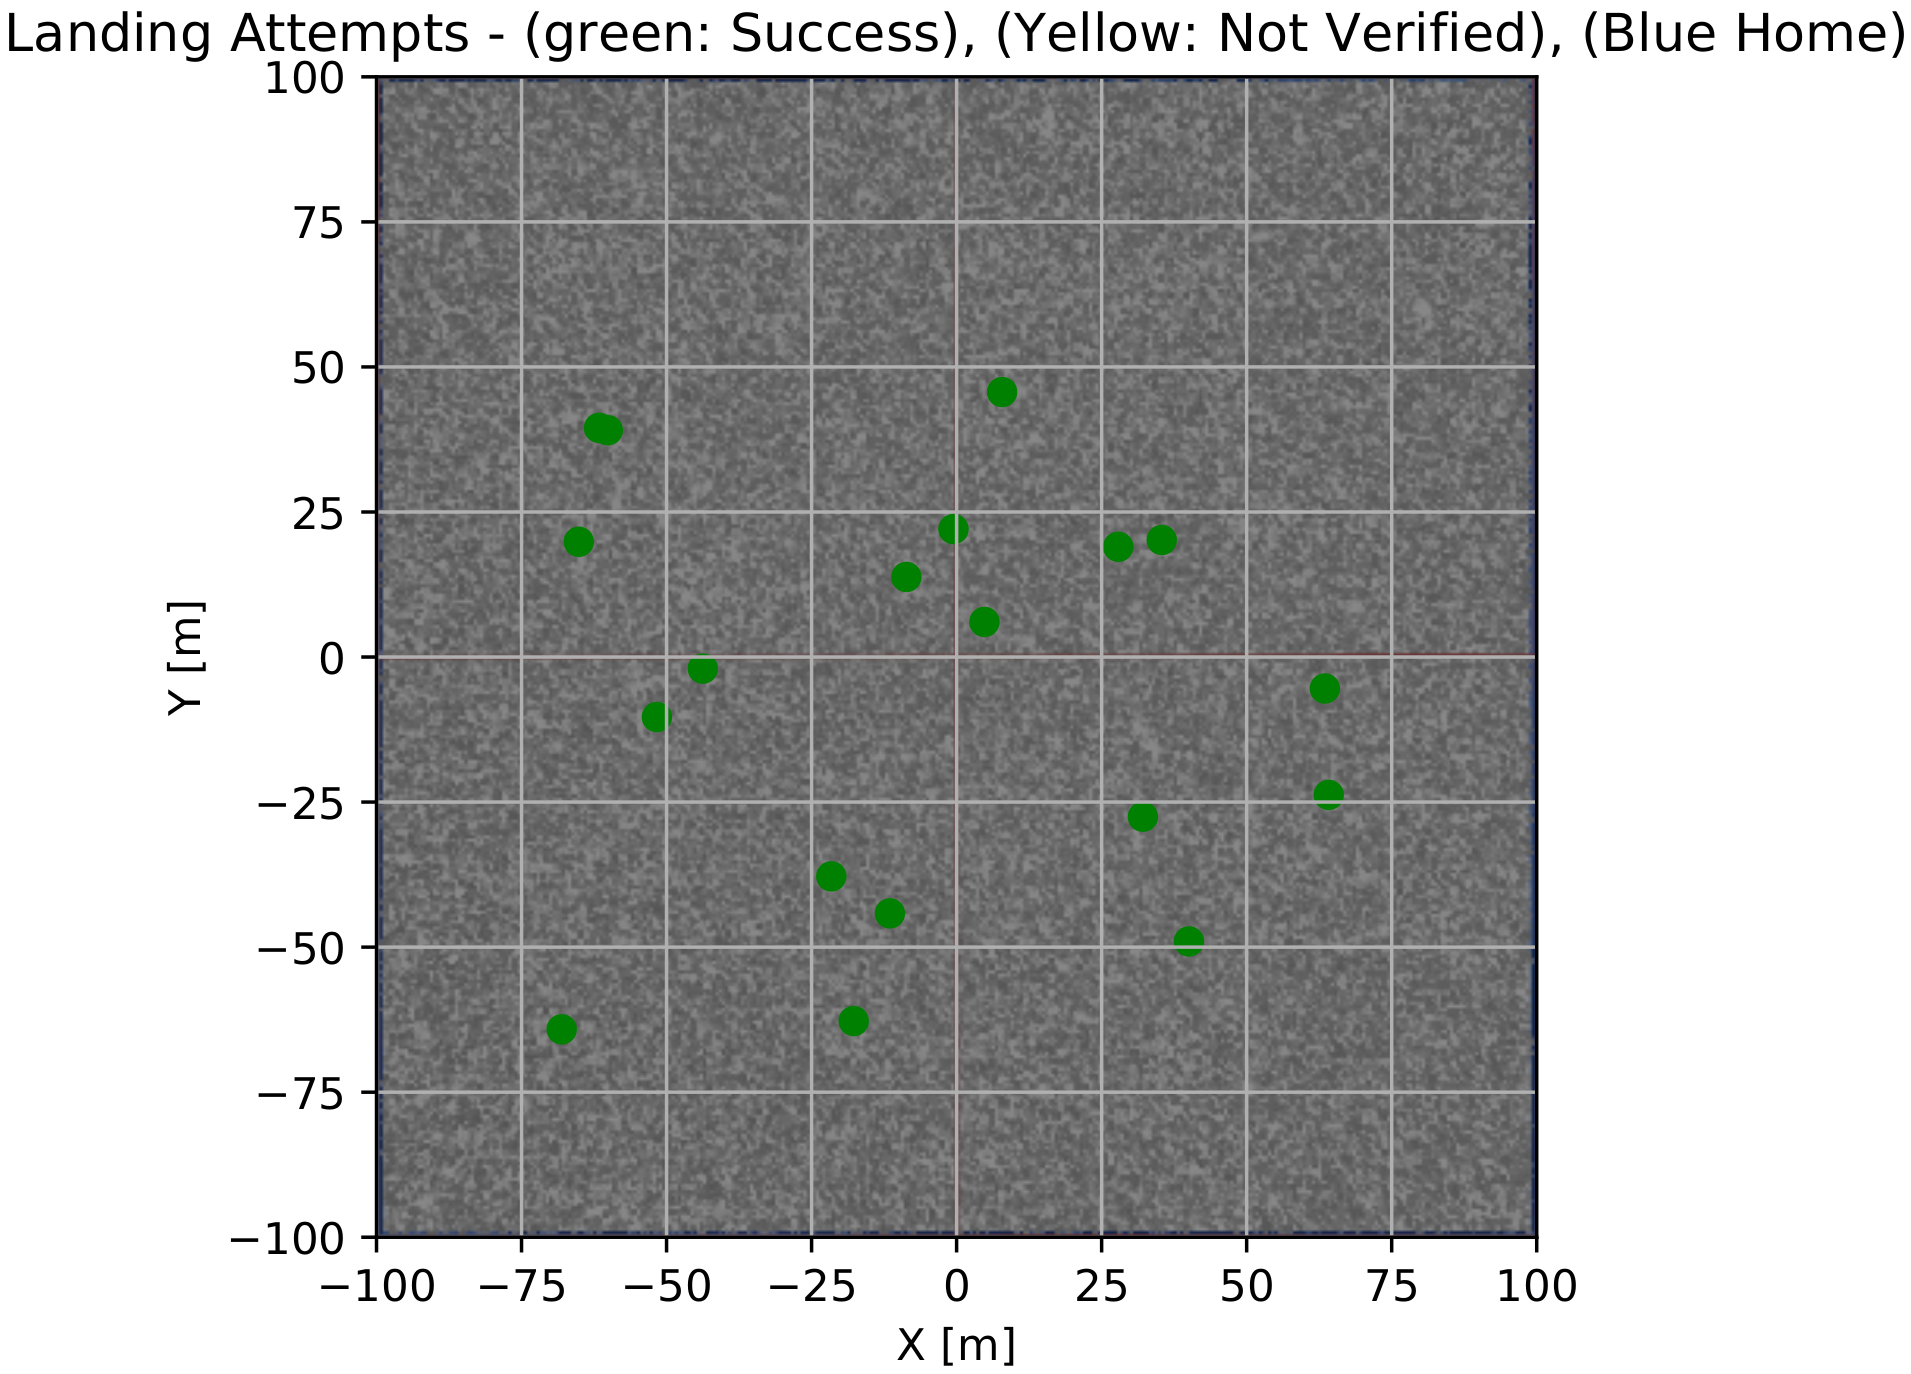
\includegraphics[scale=0.5]{images/evaluation/landing_rough_covered.png}
    \caption{Landing attempt locations for the rough map with platform covered by the mission}
    \label{fig:land_rough_covered} %TODO: replace
    \end{figure}

    As both the spawn platform and the landing platforms where spawned randomly, evaluating the visual outcome is redundant. For sake of completion however, it is still displayed.

    \subsubsection{Numerical Discussion}
    One timeout occurred, but each attempt at landing resulted in a success. 

    This proves that LSD does in fact not perceive convincing landing sites where there should be none. Additionally, as the drone never went home, this proves that LSD also detects landing sites where there should be safe landing zones.
    
    Each landing site selected was verified. This convincing result is not surprising as the inserted landing sites are perfect landing sites and are therefore unlikely to trigger a verification failure.

\section{Theoretical Edge Cases}
\cref{sec:test_flights} shows that the implemented landing procedure performs well only terrain that is roughly comparable to that on Mars. These tests represent rather ordinary cases though. In the following, a number of theoretical edge cases are introduced and their handling by this work's pipeline discussed.

\subsection{Arrival on Mars}
One concept for the rotorcraft arrival on Mars is its takeoff during the descent of the main payload. In the Mars Sample Return mission which has since been aborted for instance, this payload would have been the landing platform to return the Mars samples to. From that lander the rotorcraft would take off mid-descent and land on its own.

Playing this scenario through, a small mission or pattern needs to be flown in order to move laterally and thus detect landing sites. Additionally, as the platform from which we took off is descending with neck-breaking velocity, we need to consider a different location for the choice of our home position. This can be done prior to the flight using a mixture of HiRISE orbiter images and information provided by Opportunity and Ingenuity. The ladder two options also ensure a sufficient image resolution to safely determine a home position.

In case of successful landing site detection during this mission, the landing procedure is initiated as usual. If no candidates for suitable landing areas were found however, further landing site search patterns at random locations are flown. If the landing site buffer remains empty still, the aforementioned synthetic home position is navigated to and landed at.

\subsection{Flying on Large Scale Inclined Terrain}
The tests performed all happened on generally even terrain with rough and inclined areas spread throughout. What happens however, when we want to fly the drone over large scale inclined terrain? An example of this could be flying out of the Jezero crater which is where the Opportunity rover was deployed.

In this case, the necessary precautions must be taken during the mission planning stage. Assuming a mission was created at a cruise altitude high enough to allow lateral traversal to the farthest mission waypoint without danger of collision, the landing behavior would be the same. 

Two possible break points exist however:

\begin{itemize}
    \item Lack of number and quality of landing sites

    On inclined terrain fewer landing sites are detected. Secondly, a blind spot of the pipeline are unstable landing sites like larger rocks. Though the probability of landing on such a rock and thus making it fall over are very small, they exist. Even more so on inclined terrain.

    \item Collision danger when flying LS search patterns

    The mission waypoints are set deterministically. Therefore, the terrain can be accounted for during their creation. 
    
    This is not the case for the random flight patterns execute when no landing sites are available. The center point of a rectangular search pattern is set randomly at a fixed distance from the location where the action was invoked. If during the mission a landing site was found at a very high altitude and turned out to be a false candidate, the LS search is initiated at that location. This case is schematically depicted in \cref{fig:search_pattern_collision}. Note how the found landing site was detected at a significant distance from the last mission waypoint. 

    \begin{figure}[h]
        \centering
        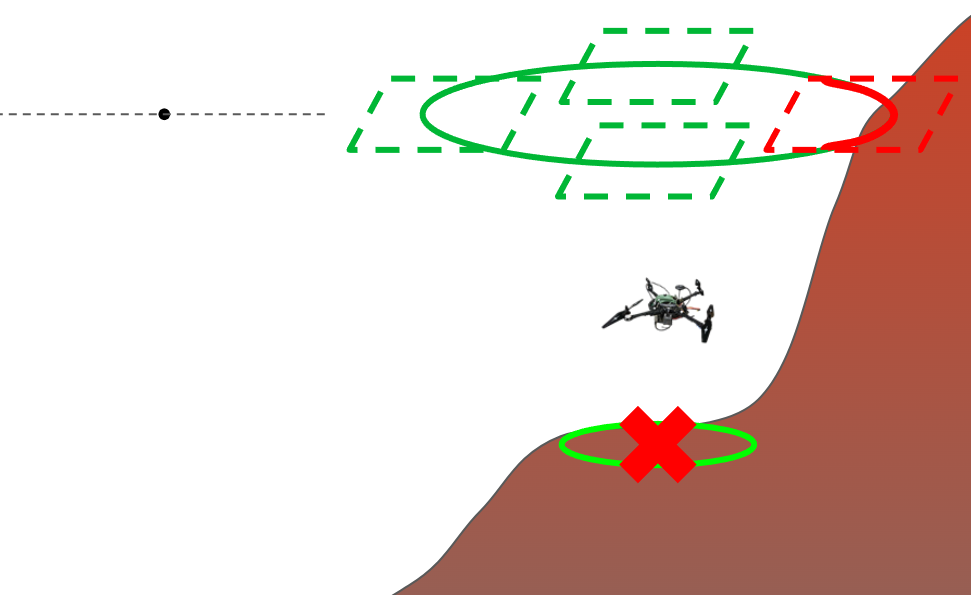
\includegraphics[scale=0.35]{images/evaluation/search_pattern_collision.png}
        \caption{Break case of landing site search pattern. The black dot indicates the last mission waypoint at cruise altitude. The bright green circle with the red cross show an invalid landing site and the circle above the drone shows the possible center points of search patterns.}
        \label{fig:search_pattern_collision}
    \end{figure}
\end{itemize}

One more break case for the presented pipeline is overhanging terrain. In that case the ascent to a clearing altitude does not constitute a safe approach.

It has to be noted that the exploration of terrain as advanced as overhanging ground and cave systems is not considered part of the LORNA endeavor.